\documentclass{standalone}
\usepackage{tikz}

%x step={
\usetikzlibrary{fit}
%x }

\begin{document}

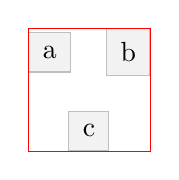
\begin{tikzpicture}
%x description="node positioning"
	\begin{scope}[every node/.style={fill=gray!10, draw=gray!50, inner sep=5}]
		\node (a) at (0,1) {a};
		\node (b) at (1,1) {b};
		\node (c) at (0.5, 0) {c};
	\end{scope}
%x step={
	\node [draw=red, rectangle, 
		fit=(a)(b)(c), inner sep=0
		] {};
%x }
\end{tikzpicture}

\end{document}
